\documentclass{../acm_proc_article-me11_tweaked}
\usepackage[usenames,dvipsnames,svgnames,table]{xcolor}
\usepackage[sort&compress,numbers]{natbib}

\def \rothead [#1]{\rotatebox[origin=l]{60}{#1}}
\renewcommand{\arraystretch}{1.5}

\begin{document}

\conferenceinfo{\textit{MediaEval 2013 Workshop,}}{October 18-19, 2013, Barcelona, Spain}

\title{Identifying the Geographic Location of an Image with a Multimodal Probability Density Function}

%
\def\sharedaffiliation{%
\end{tabular}
\begin{tabular}{c}}
%

\numberofauthors{8}
\author{
\alignauthor
Jamie Davies\\
    \email{jagd1g11@ecs.soton.ac.uk}
\and
\alignauthor
Jonathon S. Hare\\
    \email{jsh2@ecs.soton.ac.uk}
\and
\alignauthor
Sina Samangooei\\
    \email{ss@ecs.soton.ac.uk}
\and
\alignauthor
John Preston\\
    \email{jlp1g11@ecs.soton.ac.uk}
\and
\alignauthor
Neha Jain\\
    \email{nj1g12@ecs.soton.ac.uk}
\and
\alignauthor
David P. Dupplaw
    \email{dpd@ecs.soton.ac.uk}
\sharedaffiliation
    \affaddr{Electronics and Computer Science, University of Southampton, United Kingdom}
}

\additionalauthors{Additional author: Paul H. Lewis (
email: {\texttt{phl@ecs.soton.ac.uk}})}

\maketitle
\begin{abstract}
Knowing the location that a photograph was taken provides us with data that could be useful in a wide spectrum of applications. With the advance of digital cameras, and with many users exchanging their digital cameras for their GPS-enabled mobile phones, photographs annotated with geographical locations are becoming ever more present on photo-sharing websites such as Flickr. However there is still a wide majority of online content that is not geotagged, meaning that algorithms for efficient and accurate geographical estimation of an image are needed. We present a general model for using both textual metadata and visual features of photos to automatically place them on a world map. This forms the University of Southampton's entry for the MediaEval 2013 Placing task.
\end{abstract}

\keywords{Geotagging, Probability Density, Image Annotation}

\section{Introduction and Motivation}
The primary goal of the 2013 MediaEval placing task~\cite{mediaevalPlacing13} was to develop techniques for accurately predicting the geo-location of a set of Flickr images in terms of latitude and longitude. In addition, a secondary goal was to enhance predictions by estimating the error of the predicted location of each image. The task organisers provided a set of about 8.5 million images with metadata and locations for training, and a set of 262,000 images without geotags for testing.

The motivation for the techniques we have developed for the task was twofold; we firstly wanted to develop a technique that can operated using either the visual content or the metadata, but which also seamlessly allowed blending of information across modalities and also allowed information from external gazetteers to incorporated. Secondly, we wanted the technique to be scalable and efficient, with the aim of being able to estimate the position of an image in well under a second using standard desktop hardware.

\section{Overall Methodology}
The basic idea of our approach is that we estimate a continuous probability density function (PDF) over the surface of the Earth from a number of \emph{features} extracted from the query image and/or its metadata. To estimate the PDF, each feature provides a fixed size set of \emph{points} (in terms of latitude and longitude) which are then combined (Figure~\ref{fig:features}), and a kernel density estimator (Parzen Window)~\cite{parzen1962estimation} can be used to estimate the probability density at any arbitrary position (Figure~\ref{fig:density}). By finding the modes of the PDF we create an estimate the location of the photograph from the position of the mode with the highest probability. By fitting a univariate Gaussian over the support of the highest probability mode, we can estimate the accuracy of the estimated geolocation as a function of the variance of the Gaussian.

\begin{figure}
	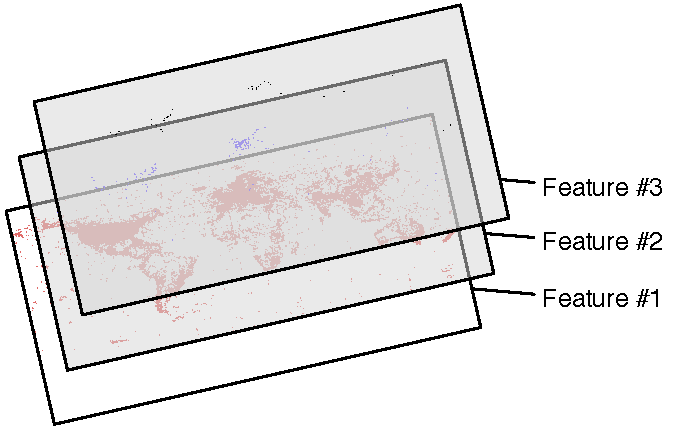
\includegraphics[width=\columnwidth]{images/layers}
	\caption{\label{fig:features}Sets of points representing the probability density of each feature are overlaid.}
\end{figure}

\begin{figure}
	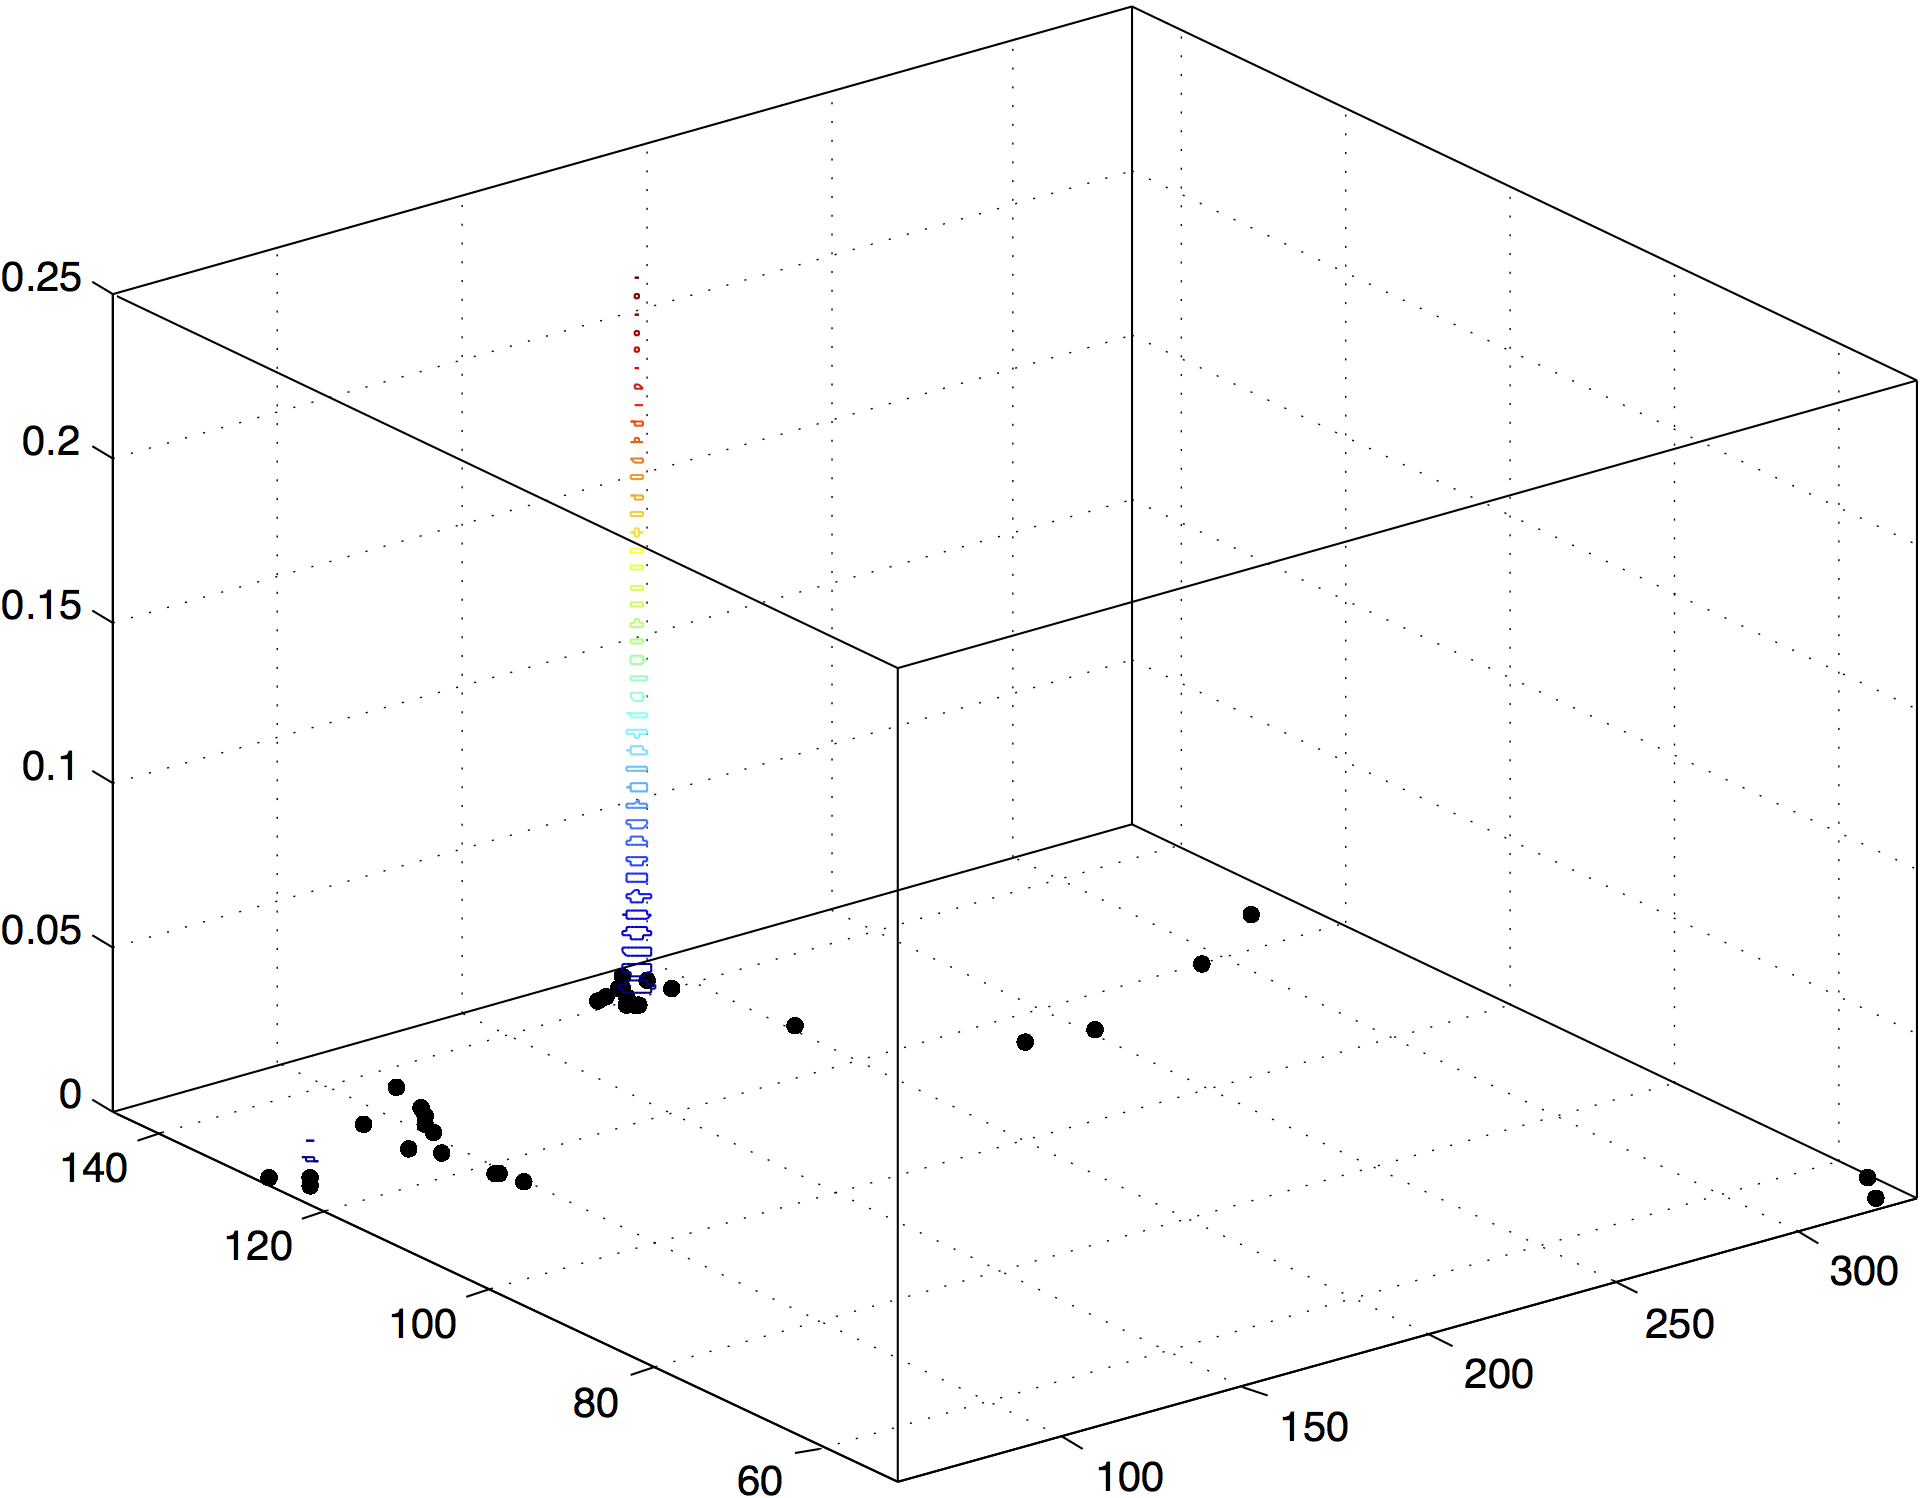
\includegraphics[width=\columnwidth]{images/density}
	\caption{\label{fig:density}A kernel density estimator is applied and we estimate the photograph's location at the position of the largest peak in the density function.}
\end{figure}

In practice, density estimation and mode-finding can be combined by applying the mean-shift algorithm~\cite{1000236}. Mean-shift has been used in the context of geolocation estimation in the past; \citeauthor{Crandall:2009:MWP:1526709.1526812} used mean-shift to determine landmarks, and \citeauthor{Hays:2008:im2gps} used mean-shift on the results of content-based image search to determine probable locations. Whilst \citeauthor{Hays:2008:im2gps}'s approach is similar to ours, it differs in a number of important ways. In particular, whereas \citeauthor{Hays:2008:im2gps} only considered single (high recall/low precision) content-based features, we consider the fusion of multiple features from different modalities. \citeauthor{Hays:2008:im2gps} used the mean-shift algorithm for coarse-grained location estimation, with a very large kernel bandwidth. In our technique, because of the way we're using features we're able to use a much smaller kernel bandwidth for fine-grained location estimation.

\section{Experiments}
\subsection{Features}
\textcolor{red}{\begin{itemize}
    \item Mention all features we tried
    \item Time $\rightarrow$ better?
    \item VLAD $\rightarrow$ similar to CEDD?
    \item LSH query expansion $\rightarrow$ too slow, not much better
\end{itemize}}

\subsection{Runs}
See table \ref{tab:runconf} for details on the configuration of the run submissions.
\begin{table}
    \centering
    \begin{tabular}[h]{l|*{5}{>{\centering\arraybackslash}m{0.85cm}|}}
        \multicolumn{1}{c}{} & \multicolumn{1}{c}{\rothead[Prior]} & \multicolumn{1}{c}{\rothead[Tags]} & \multicolumn{1}{c}{\rothead[CEDD]} & \multicolumn{1}{c}{\rothead[SIFT-LSH]} & \multicolumn{1}{c}{\rothead[Geonames]} \\
        \hline
        Run 1 & \checkmark & \checkmark & \checkmark & \checkmark & \\
        \hline
        Run 2 & \checkmark & & \checkmark & \checkmark & \\
        \hline
        Run 3 & \checkmark & \checkmark & & & \\
        \hline
        Run 4 & \checkmark & \checkmark & & \checkmark & \\
        \hline
        Run 5 & \checkmark & \checkmark & \checkmark & \checkmark & \checkmark \\
        \hline
    \end{tabular}
    \caption{The feature configuration for the run submissions.}
    \label{tab:runconf}
\end{table}

\subsubsection{Run 1: Text+Visual, provided data}
\subsubsection{Run 2: Visual only, provided data}
\subsubsection{Run 3: Text only, provided data}
\subsubsection{Run 4: Text+Visual, bigger dataset}
\subsubsection{Run 5: Text+Visual, provided data with tag boosting}
\subsection{Results and Discussion}

\section{Conclusions and Future Work}
\textcolor{red}{\begin{itemize}
    \item LSH query expansion
    \item Geonames
    \item VLAD
    \item GIST
    \item More features
\end{itemize}}

\section{Acknowledgments}
The described work was funded by the European Union Seventh Framework Programme (FP7/2007-2013) under grant agreements 270239 (ARCOMEM), and 287863 (TrendMiner).


\bibliographystyle{abbrv}
\bibliography{../bibliography}
\end{document}
